\begin{figure*}[t]
  \centering
  \begin{subfigure}{0pt}\phantomsubcaption\label{fig:props-p1}\end{subfigure}%
  \begin{subfigure}{0pt}\phantomsubcaption\label{fig:props-p2}\end{subfigure}%
  \begin{subfigure}{0pt}\phantomsubcaption\label{fig:props-p3}\end{subfigure}%
  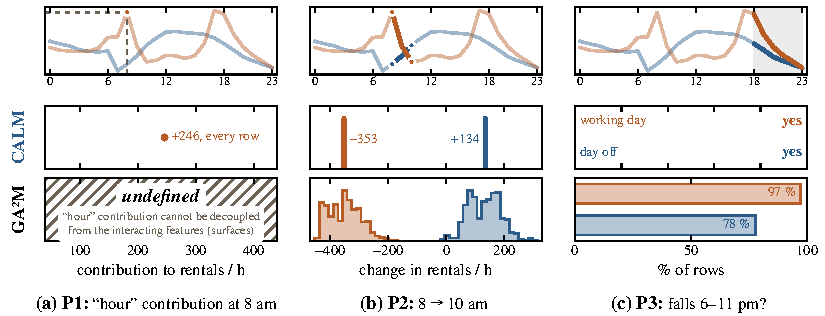
\includegraphics[width=\linewidth]{images/bike/props}
  \caption{The three properties on the model of Figure~\ref{fig:hero}, each asked on every row of the data. Top: CALM's curves, the question marked. CALM's answers are read by eye; the \gamm's are computed, each of the 17{,}379 rows through its eight terms with the hour.
    (\subref{fig:props-p1}) The hour's contribution at 8\,am on a working day: CALM reads $+246$ off the working-day curve, the same on every row; the \gamm's is undefined, since the hour's contribution cannot be decoupled from the interacting features (its seven surfaces).
    (\subref{fig:props-p2}) $\hat{y}(10\,\text{am}) - \hat{y}(8\,\text{am})$: CALM $-353$ on working days and $+134$ on days off, exact on every row since no dotted line is crossed; the \gamm{} spreads from $-430$ to $-257$ and from $+54$ to $+215$ (5th--95th percentile).
    (\subref{fig:props-p3}) Does the prediction fall every hour from 6\,pm to 11\,pm? CALM: yes on working days and days off, since both curves fall and cross no dotted line; the \gamm: on 97\% of working days and 78\% of days off.}
  \label{fig:props}
\end{figure*}
